\documentclass[aspectratio=169,11pt]{beamer}
\usepackage{fontspec}
\setmainfont{Noto Sans CJK SC}
\setsansfont{Noto Sans CJK SC}
\renewcommand{\familydefault}{\sfdefault}
\usefonttheme{professionalfonts}
\usetheme{Boadilla}
\setbeamertemplate{navigation symbols}{}
\setbeamertemplate{footline}[frame number]
\setbeamertemplate{itemize item}{\small$\blacktriangleright$}
\usepackage{graphicx}
\usepackage{booktabs}
\usepackage{amsmath}
\usepackage{xcolor}
\usepackage{tikz}
\usetikzlibrary{positioning,arrows.meta}

\graphicspath{{assets/}}

\definecolor{MainBlue}{HTML}{1F3A5F}
\definecolor{SoftBlue}{HTML}{EAF2FB}
\definecolor{SoftOrange}{HTML}{FFF1E6}
\definecolor{SoftGray}{HTML}{F5F7FA}

\setbeamercolor{title}{fg=MainBlue}
\setbeamercolor{frametitle}{fg=MainBlue}
\setbeamerfont{title}{series=\bfseries,size=\Large}
\setbeamerfont{frametitle}{series=\bfseries,size=\large}

\title{高红移 UVLF}
\subtitle{SSP 卷积方案对跨红移 UVLF 拟合结果的影响}
\author{朱厚瑞}
\date{\today}

\begin{document}

\begin{frame}
  \titlepage
\end{frame}

\begin{frame}{当前状态}
\centering
\resizebox{0.96\linewidth}{!}{
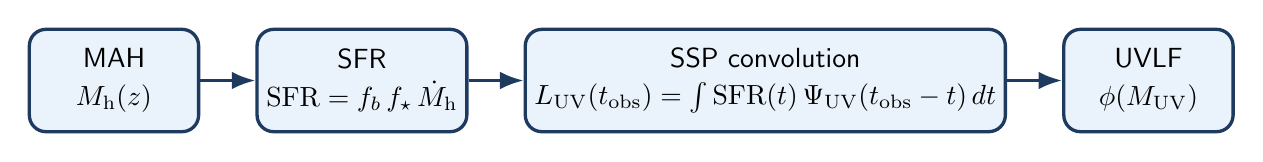
\begin{tikzpicture}[
  node distance=0.9cm and 0.7cm,
  box/.style={draw=MainBlue, very thick, rounded corners=6pt, fill=SoftBlue,
    minimum width=2.15cm, minimum height=1.30cm, align=center, font=\normalsize},
  arr/.style={-{Latex[length=3mm]}, very thick, draw=MainBlue}
]
  \node[box] (mah) {MAH\\[0.15em]$M_{\rm h}(z)$};
  \node[box, right=of mah] (sfr) {SFR\\[0.15em]${\rm SFR}=f_b\,f_\star\,\dot M_{\rm h}$};
  \node[box, right=of sfr, minimum width=3.70cm] (ssp) {SSP convolution\\[0.15em]$L_{\rm UV}(t_{\rm obs})=\int {\rm SFR}(t)\,\Psi_{\rm UV}(t_{\rm obs}-t)\,dt$};
  \node[box, right=of ssp] (uvlf) {UVLF\\[0.15em]$\phi(M_{\rm UV})$};

  \draw[arr] (mah) -- (sfr);
  \draw[arr] (sfr) -- (ssp);
  \draw[arr] (ssp) -- (uvlf);
\end{tikzpicture}
}

\vspace{0.8em}

\normalsize
MAH 采用 McBride et al. (2009) 参数化，并对 \(\beta,\gamma\) 做 Monte Carlo 采样。

\vspace{0.3em}

\begin{minipage}{0.9\linewidth}
\centering
\large
\[
M_{\rm h}(z)=M_{\rm h,obs}\left(\frac{1+z}{1+z_{\rm obs}}\right)^\beta
\exp\!\left[-\gamma\,(z-z_{\rm obs})\right]
\]
\[
f_\star(M)=\frac{2\epsilon_0}{(M/M_c)^{-\beta_\star}+(M/M_c)^{\gamma_\star}}
\]
\end{minipage}
\end{frame}

\begin{frame}{关键量化结果}
\begin{columns}[T,onlytextwidth]
  \column{0.56\textwidth}
  \centering
  \Large
  \[
  \begin{array}{c|c}
  z & L_{\mathrm{UV,SSP}} / L_{\mathrm{UV,inst,long}} \\
  \hline
  6 & 1.27\text{--}1.29 \\
  8 & 0.82\text{--}0.84 \\
  10 & 0.64\text{--}0.67 \\
  12.5 & 0.56\text{--}0.59
  \end{array}
  \]

  \column{0.40\textwidth}
  \begin{beamercolorbox}[rounded=true, sep=0.65em, wd=\linewidth]{block body}
    \Large
    \textbf{瞬时 UV 基准}\\[0.3em]
    \centering
    \Large
    $\mathrm{SFR}(z_{\rm obs}) / K_{\rm UV,SSP,long}$\\[0.8em]
    \normalsize
    $K_{\rm UV,SSP,long} \approx 6.1\times10^{-29}$
  \end{beamercolorbox}
\end{columns}

\vspace{0.8em}

\begin{beamercolorbox}[rounded=true, sep=0.8em, wd=0.94\linewidth, center]{block body}
  \normalsize
  \textbf{关键信号：}
  SSP 的有效 UV 记忆时间主要集中在 \(30\)–\(100\,\mathrm{Myr}\)；
  低 \(z\) 更接近稳态，高 \(z\) 明显偏离稳态。
\end{beamercolorbox}
\end{frame}

\begin{frame}{Intrinsic UV：单个 halo 的计算}
\begin{columns}[T,onlytextwidth]
  \column{0.54\textwidth}
  \centering
  \resizebox{0.98\linewidth}{!}{
  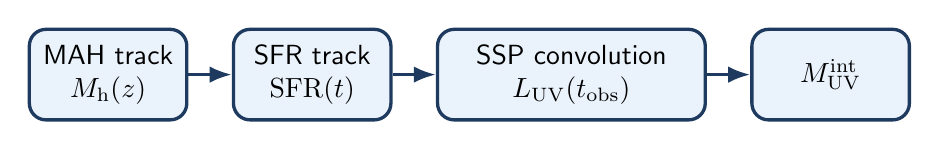
\begin{tikzpicture}[
    node distance=0.8cm and 0.55cm,
    box/.style={draw=MainBlue, very thick, rounded corners=6pt, fill=SoftBlue,
      minimum width=2.0cm, minimum height=1.15cm, align=center, font=\normalsize},
    arr/.style={-{Latex[length=2.8mm]}, very thick, draw=MainBlue}
  ]
    \node[box] (mah) {MAH track\\$M_{\rm h}(z)$};
    \node[box, right=of mah] (sfr) {SFR track\\${\rm SFR}(t)$};
    \node[box, right=of sfr, minimum width=3.4cm] (ssp) {SSP convolution\\$L_{\rm UV}(t_{\rm obs})$};
    \node[box, right=of ssp] (muv) {$M_{\rm UV}^{\rm int}$};

    \draw[arr] (mah) -- (sfr);
    \draw[arr] (sfr) -- (ssp);
    \draw[arr] (ssp) -- (muv);
  \end{tikzpicture}
  }

  \vspace{0.8em}

  \small
  \begin{itemize}
    \item 对每个终质量 \(M_{\rm h,obs}\)，抽样一组 \((\beta,\gamma)\) 生成 MAH 轨道
    \item 对每条 MAH 轨道逐时刻计算 \({\rm SFR}(t)\)
    \item 用 SSP 核对整段 SFH 卷积，得到观测时刻的 intrinsic UV
  \end{itemize}

  \column{0.43\textwidth}
  \footnotesize
  \begin{align*}
  M_{\rm h}(z)
  &= M_{\rm h,obs}
  \left(\frac{1+z}{1+z_{\rm obs}}\right)^\beta \\
  &\quad \times \exp[-\gamma(z-z_{\rm obs})]
  \end{align*}

  \begin{align*}
  f_\star(M)
  &= \frac{2\epsilon_0}
  {(M/M_c)^{-\beta_\star}+(M/M_c)^{\gamma_\star}}
  \end{align*}

  \begin{align*}
  {\rm SFR}(t)
  &= f_b\,f_\star(M_{\rm h})\,\dot M_{\rm h}
  \end{align*}

  \begin{align*}
  L_{\rm UV}(t_{\rm obs})
  &= \int {\rm SFR}(t)\,
  \Psi_{\rm UV}(t_{\rm obs}-t)\,dt
  \end{align*}

  \begin{align*}
  M_{\rm UV}^{\rm int}
  &= -2.5\log_{10}L_{\rm UV}+C
  \end{align*}
\end{columns}
\end{frame}

\begin{frame}{Intrinsic UVLF：从 halo 样本到 \(\phi(M_{\rm UV})\)}
\begin{columns}[T,onlytextwidth]
  \column{0.53\textwidth}
  \centering
  \resizebox{0.98\linewidth}{!}{
  \begin{tikzpicture}[
    node distance=0.8cm and 0.55cm,
    box/.style={draw=MainBlue, very thick, rounded corners=6pt, fill=SoftOrange,
      minimum width=2.2cm, minimum height=1.2cm, align=center, font=\normalsize},
    arr/.style={-{Latex[length=2.8mm]}, very thick, draw=MainBlue}
  ]
    \node[box] (hmf) {HMF 抽样\\$M_{{\rm h},i}$};
    \node[box, right=of hmf] (tracks) {每个质量抽\\\(n_{\rm tracks}\) 条轨道};
    \node[box, right=of tracks] (muv) {得到样本\\$M_{{\rm UV},ij}^{\rm int}$};
    \node[box, right=of muv] (hist) {加权 histogram\\$\phi(M_{\rm UV})$};

    \draw[arr] (hmf) -- (tracks);
    \draw[arr] (tracks) -- (muv);
    \draw[arr] (muv) -- (hist);
  \end{tikzpicture}
  }

  \vspace{1.0em}

  \small
  \begin{itemize}
    \item 外层按 HMF 抽样终质量 \(M_{{\rm h},i}\)
    \item 内层对每个质量生成 \(n_{\rm tracks}\) 条 MAH realization
    \item 最后按 intrinsic \(M_{\rm UV}\) 分 bin，而不是按质量分 bin
  \end{itemize}

  \column{0.44\textwidth}
  \footnotesize
  \begin{align*}
  w_i
  &= \frac{\log M_{\max}-\log M_{\min}}{N_{\rm mass}}
  \left.\frac{dn}{d\log M}\right|_{M_{{\rm h},i}}
  \end{align*}

  \begin{align*}
  w_{ij} &= \frac{w_i}{n_{\rm tracks}}
  \end{align*}

  \begin{align*}
  \phi(M_k)
  &= \frac{1}{\Delta M_k}
  \sum_{ij\in k} w_{ij}
  \end{align*}

  \begin{align*}
  \phi(M_{\rm UV})
  &= \int d\log M_{\rm h}\,
  \frac{dn}{d\log M_{\rm h}} \\
  &\quad \times P(M_{\rm UV}\mid M_{\rm h},z)
  \end{align*}

  \vspace{0.4em}
  \normalsize
  \textbf{这一页讨论的是 intrinsic UVLF，尚未加入 dust。}
\end{columns}
\end{frame}

\begin{frame}{Instant 模型：完整计算流程}
\begin{columns}[T,onlytextwidth]
  \column{0.56\textwidth}
  \centering
  \resizebox{0.99\linewidth}{!}{
  \begin{tikzpicture}[
    node distance=0.75cm and 0.45cm,
    box/.style={draw=MainBlue, very thick, rounded corners=6pt, fill=SoftGray,
      minimum width=1.95cm, minimum height=1.10cm, align=center, font=\normalsize},
    arr/.style={-{Latex[length=2.8mm]}, very thick, draw=MainBlue}
  ]
    \node[box] (hmf) {HMF 抽样\\$M_{{\rm h},i}$};
    \node[box, right=of hmf] (mah) {MAH realization\\${\rm SFR}(t)$};
    \node[box, right=of mah] (inst) {取观测时刻\\${\rm SFR}(z_{\rm obs})$};
    \node[box, right=of inst, minimum width=2.45cm] (luv) {Instant UV\\$L_{\rm UV,inst}$};
    \node[box, right=of luv] (hist) {加权 histogram\\$\phi(M_{\rm UV})$};

    \draw[arr] (hmf) -- (mah);
    \draw[arr] (mah) -- (inst);
    \draw[arr] (inst) -- (luv);
    \draw[arr] (luv) -- (hist);
  \end{tikzpicture}
  }

  \vspace{0.9em}

  \small
  \begin{itemize}
    \item 与前两页使用完全相同的 HMF 抽样、MAH realization 和质量权重
    \item 唯一变化：不做 SSP 卷积，只取观测时刻的瞬时 \({\rm SFR}(z_{\rm obs})\)
    \item 因此 `Our model` 与 `Instant` 的差异只来自 UV 标定方式，而不是 HMF/MAH 抽样
  \end{itemize}

  \column{0.40\textwidth}
  \footnotesize
  \begin{align*}
  {\rm SFR}_{\rm now}
  &= {\rm SFR}(z_{\rm obs})
  \end{align*}

  \begin{align*}
  L_{\rm UV,inst}
  &= \frac{{\rm SFR}_{\rm now}}{K_{\rm UV,SSP,long}}
  \end{align*}

  \begin{align*}
  K_{\rm UV,SSP,long}
  &\approx 6.1\times10^{-29}
  \end{align*}

  \begin{align*}
  M_{\rm UV,inst}^{\rm int}
  &= -2.5\log_{10}L_{\rm UV,inst}+C
  \end{align*}

  \begin{align*}
  \phi_{\rm inst}(M_{\rm UV})
  &= \int d\log M_{\rm h}\,
  \frac{dn}{d\log M_{\rm h}} \\
  &\quad \times P_{\rm inst}(M_{\rm UV}\mid M_{\rm h},z)
  \end{align*}
\end{columns}
\end{frame}

\begin{frame}{Intrinsic UVLF 的 halo 质量组成：\(z=6,8\)}
\begin{columns}[T,onlytextwidth]
  \column{0.49\textwidth}
  \centering
  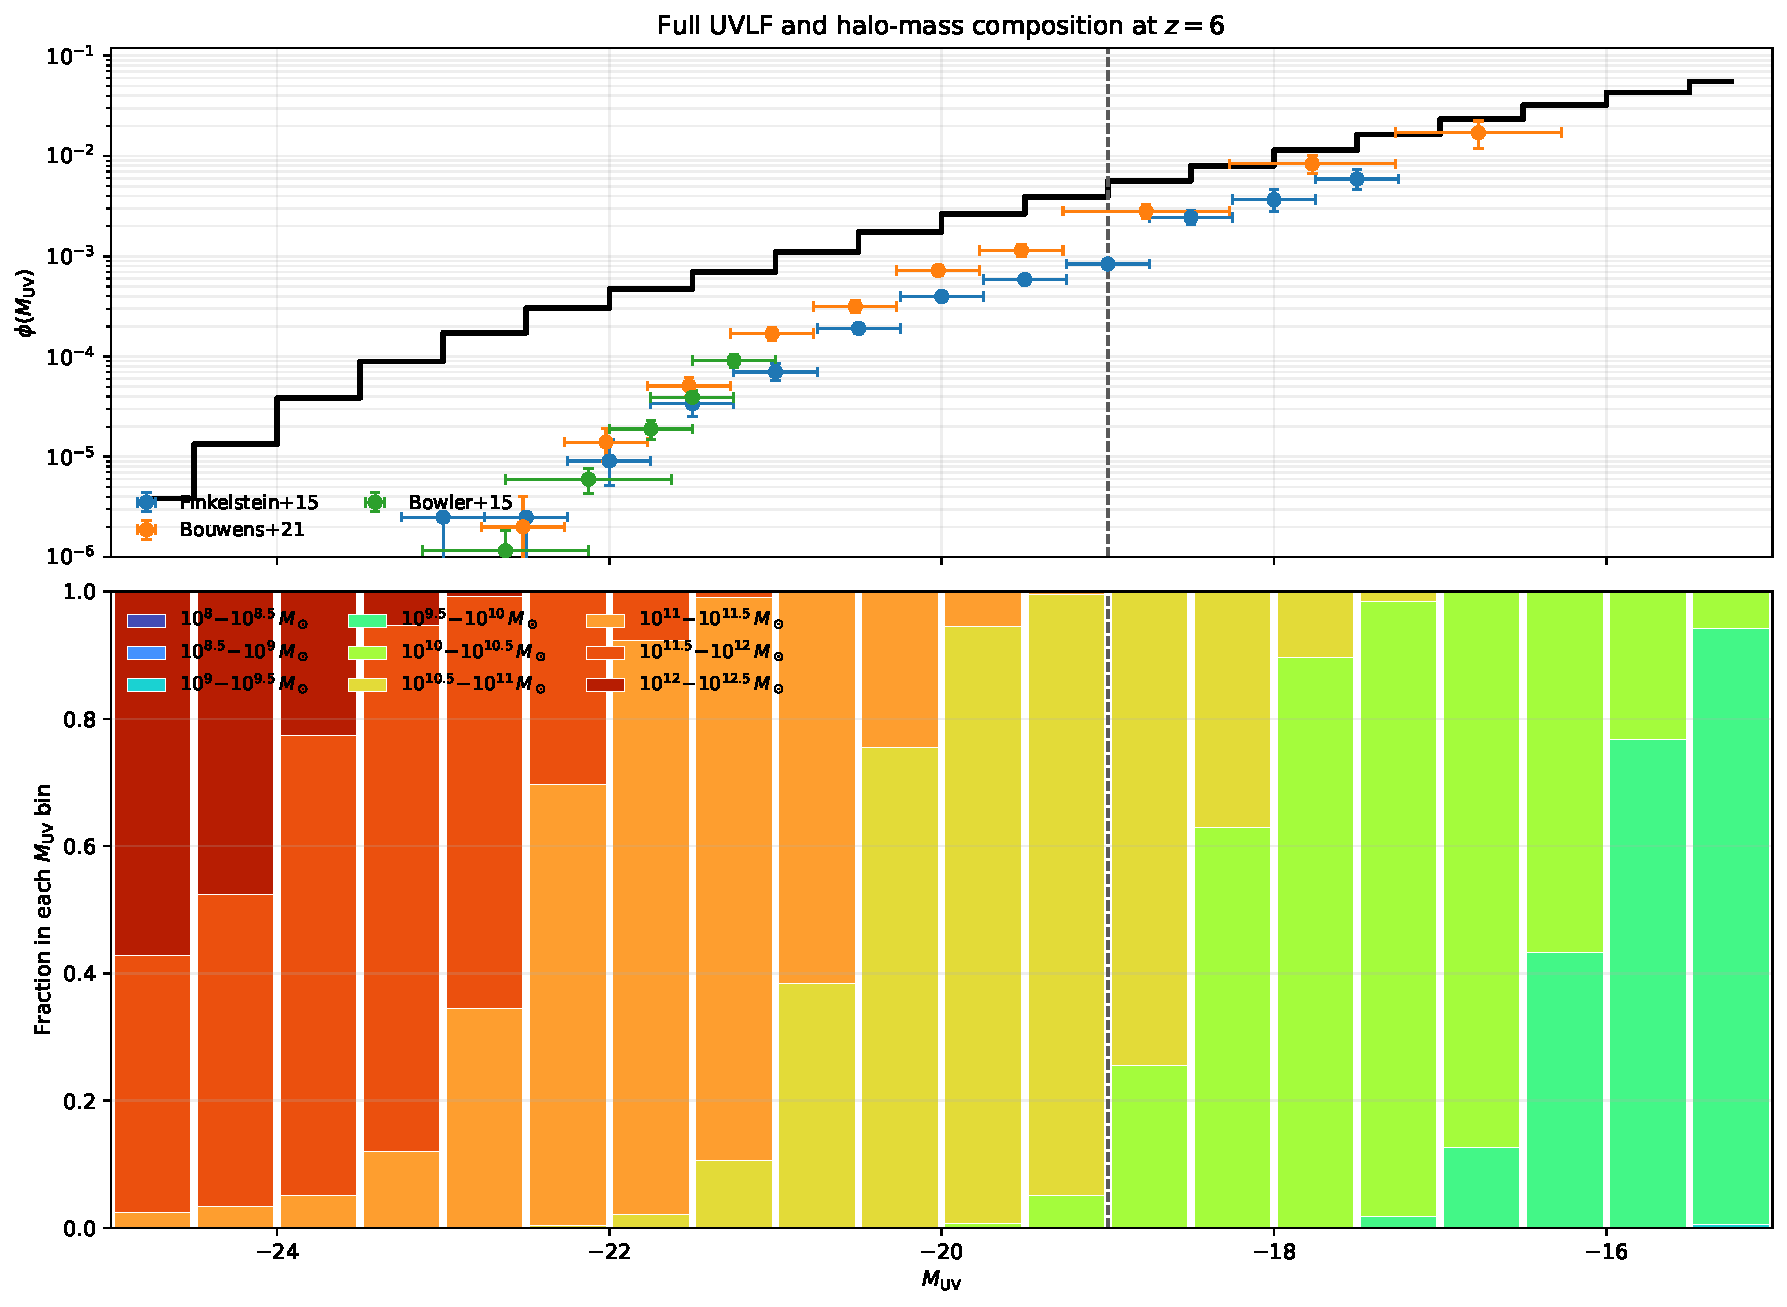
\includegraphics[width=0.98\linewidth,height=0.74\textheight,keepaspectratio]{uvlf_full_mass_composition_z6_m25_m15.pdf}

  \vspace{0.2em}
  {\large \(z=6\)}

  \column{0.49\textwidth}
  \centering
  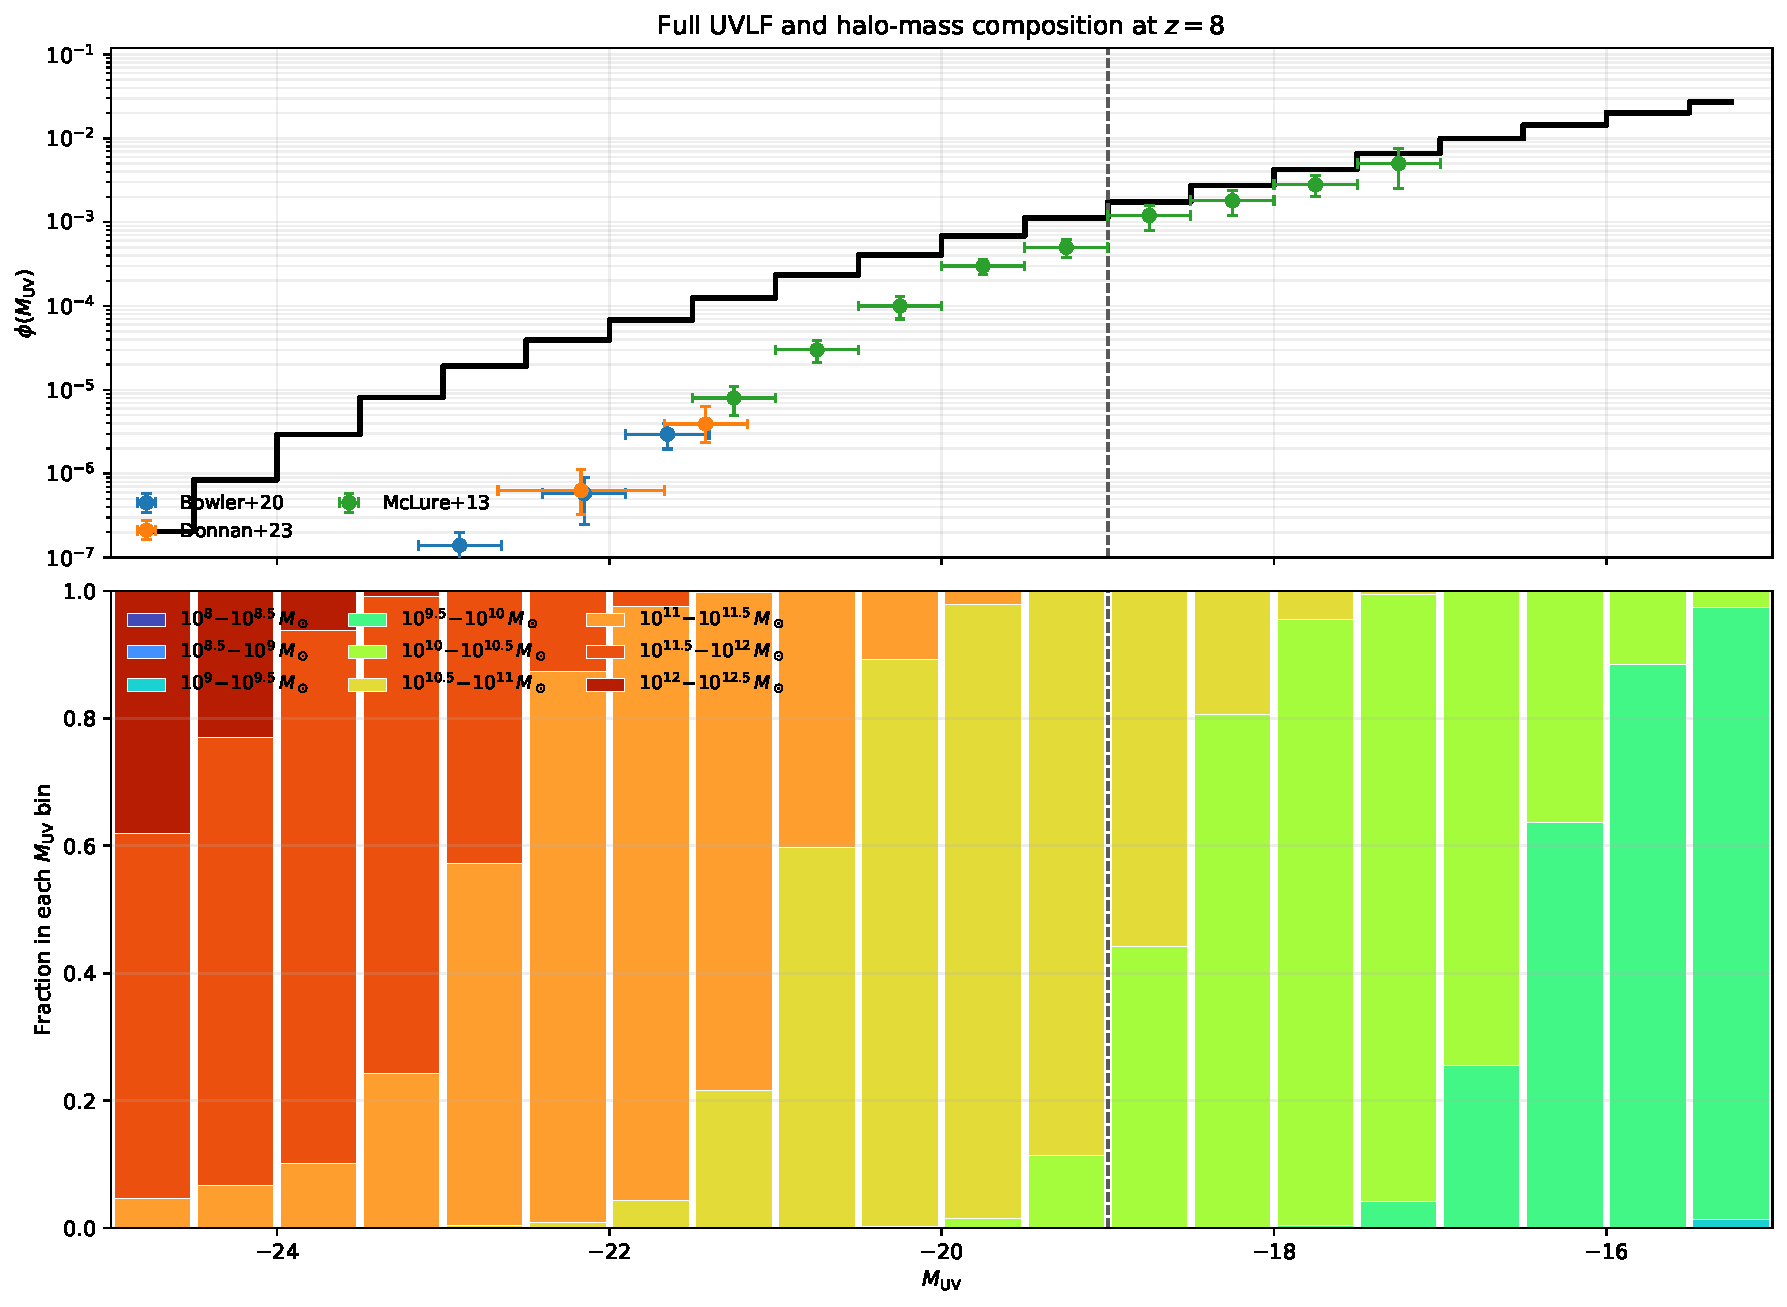
\includegraphics[width=0.98\linewidth,height=0.74\textheight,keepaspectratio]{uvlf_full_mass_composition_z8_m25_m15.pdf}

  \vspace{0.2em}
  {\large \(z=8\)}
\end{columns}
\end{frame}

\begin{frame}{Intrinsic UVLF 的 halo 质量组成：\(z=10,12.5\)}
\begin{columns}[T,onlytextwidth]
  \column{0.49\textwidth}
  \centering
  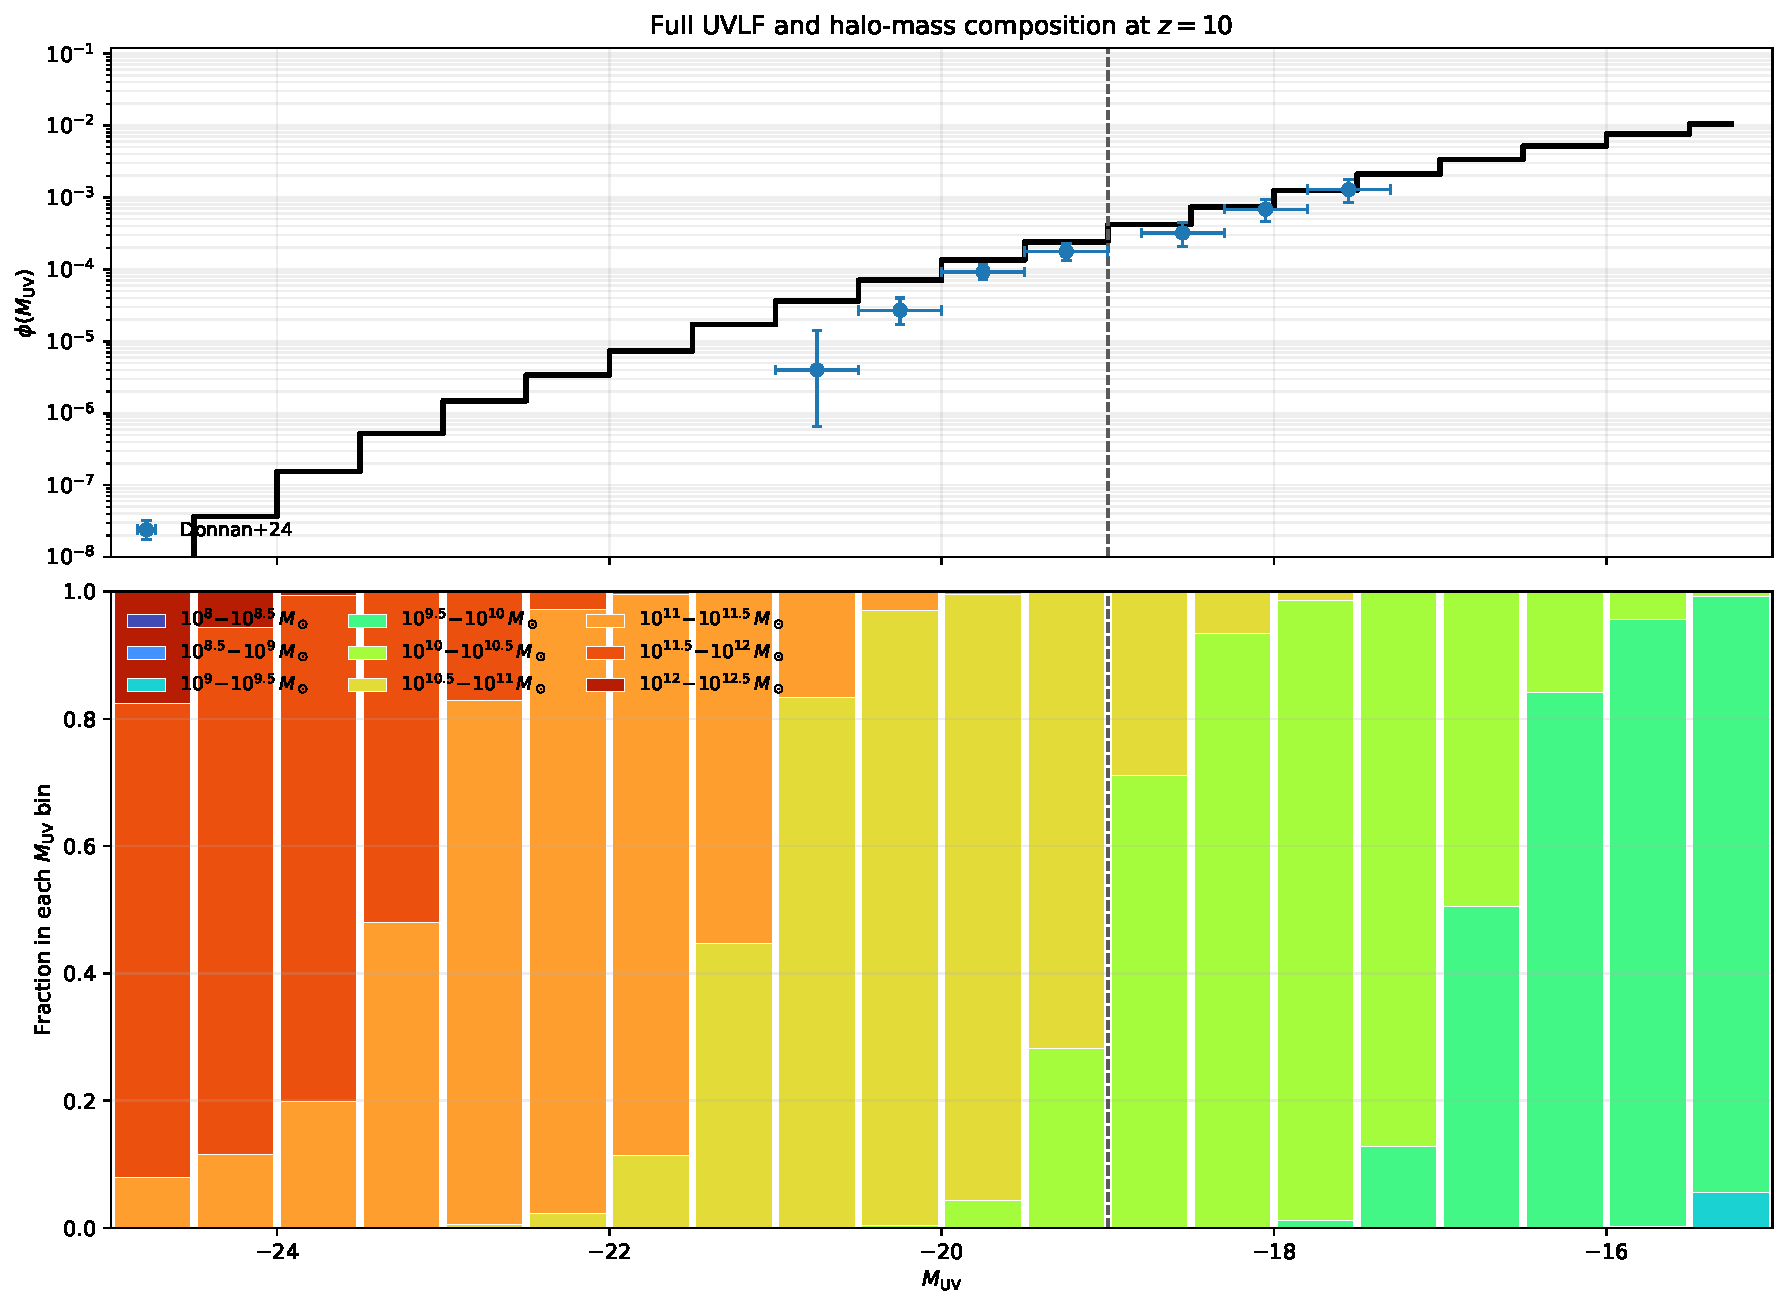
\includegraphics[width=0.98\linewidth,height=0.74\textheight,keepaspectratio]{uvlf_full_mass_composition_z10_m25_m15.pdf}

  \vspace{0.2em}
  {\large \(z=10\)}

  \column{0.49\textwidth}
  \centering
  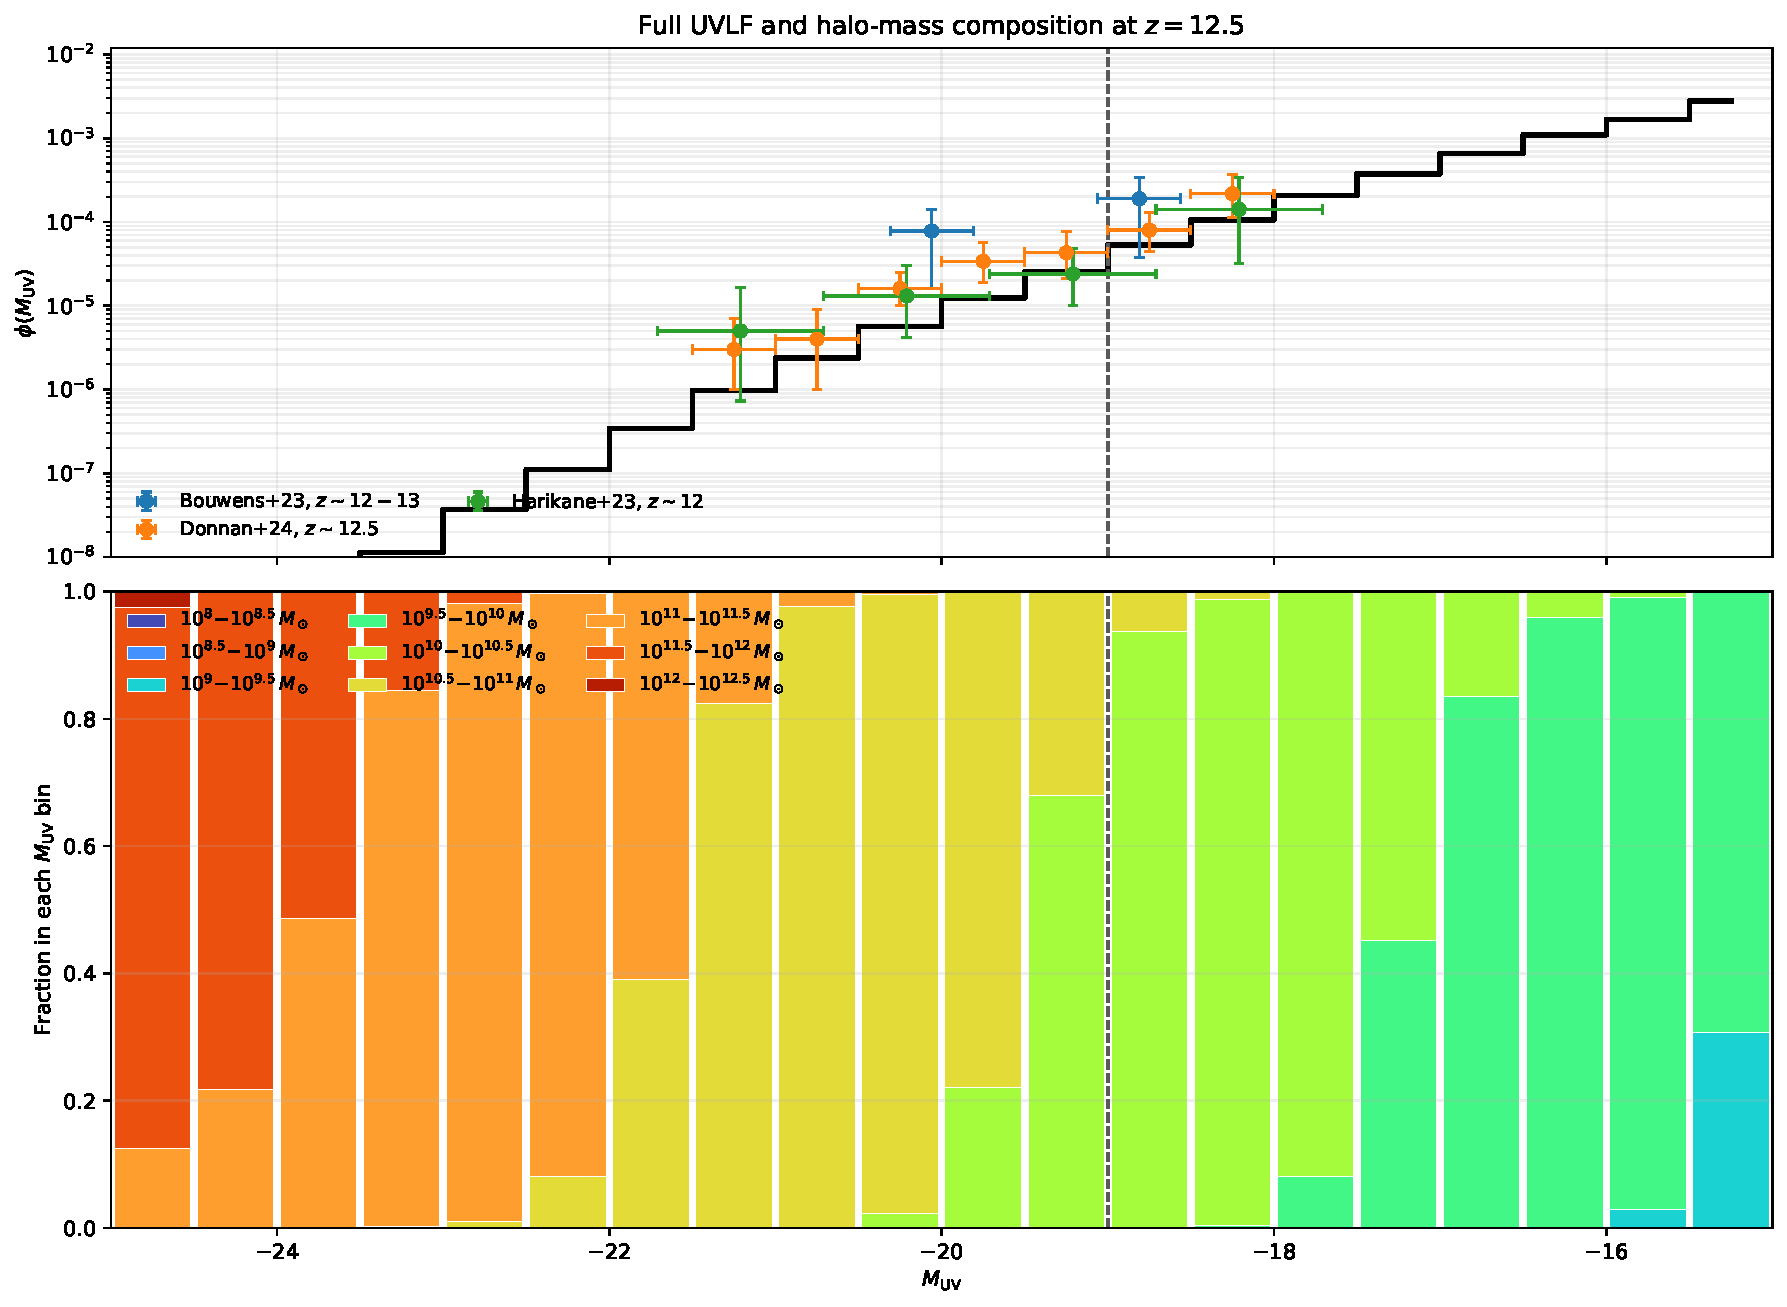
\includegraphics[width=0.98\linewidth,height=0.74\textheight,keepaspectratio]{uvlf_full_mass_composition_z12p5_m25_m15.pdf}

  \vspace{0.2em}
  {\large \(z=12.5\)}
\end{columns}
\end{frame}

\begin{frame}{同参数对比：\(z=6,8\)}
\begin{columns}[T,onlytextwidth]
  \column{0.5\textwidth}
  \centering
  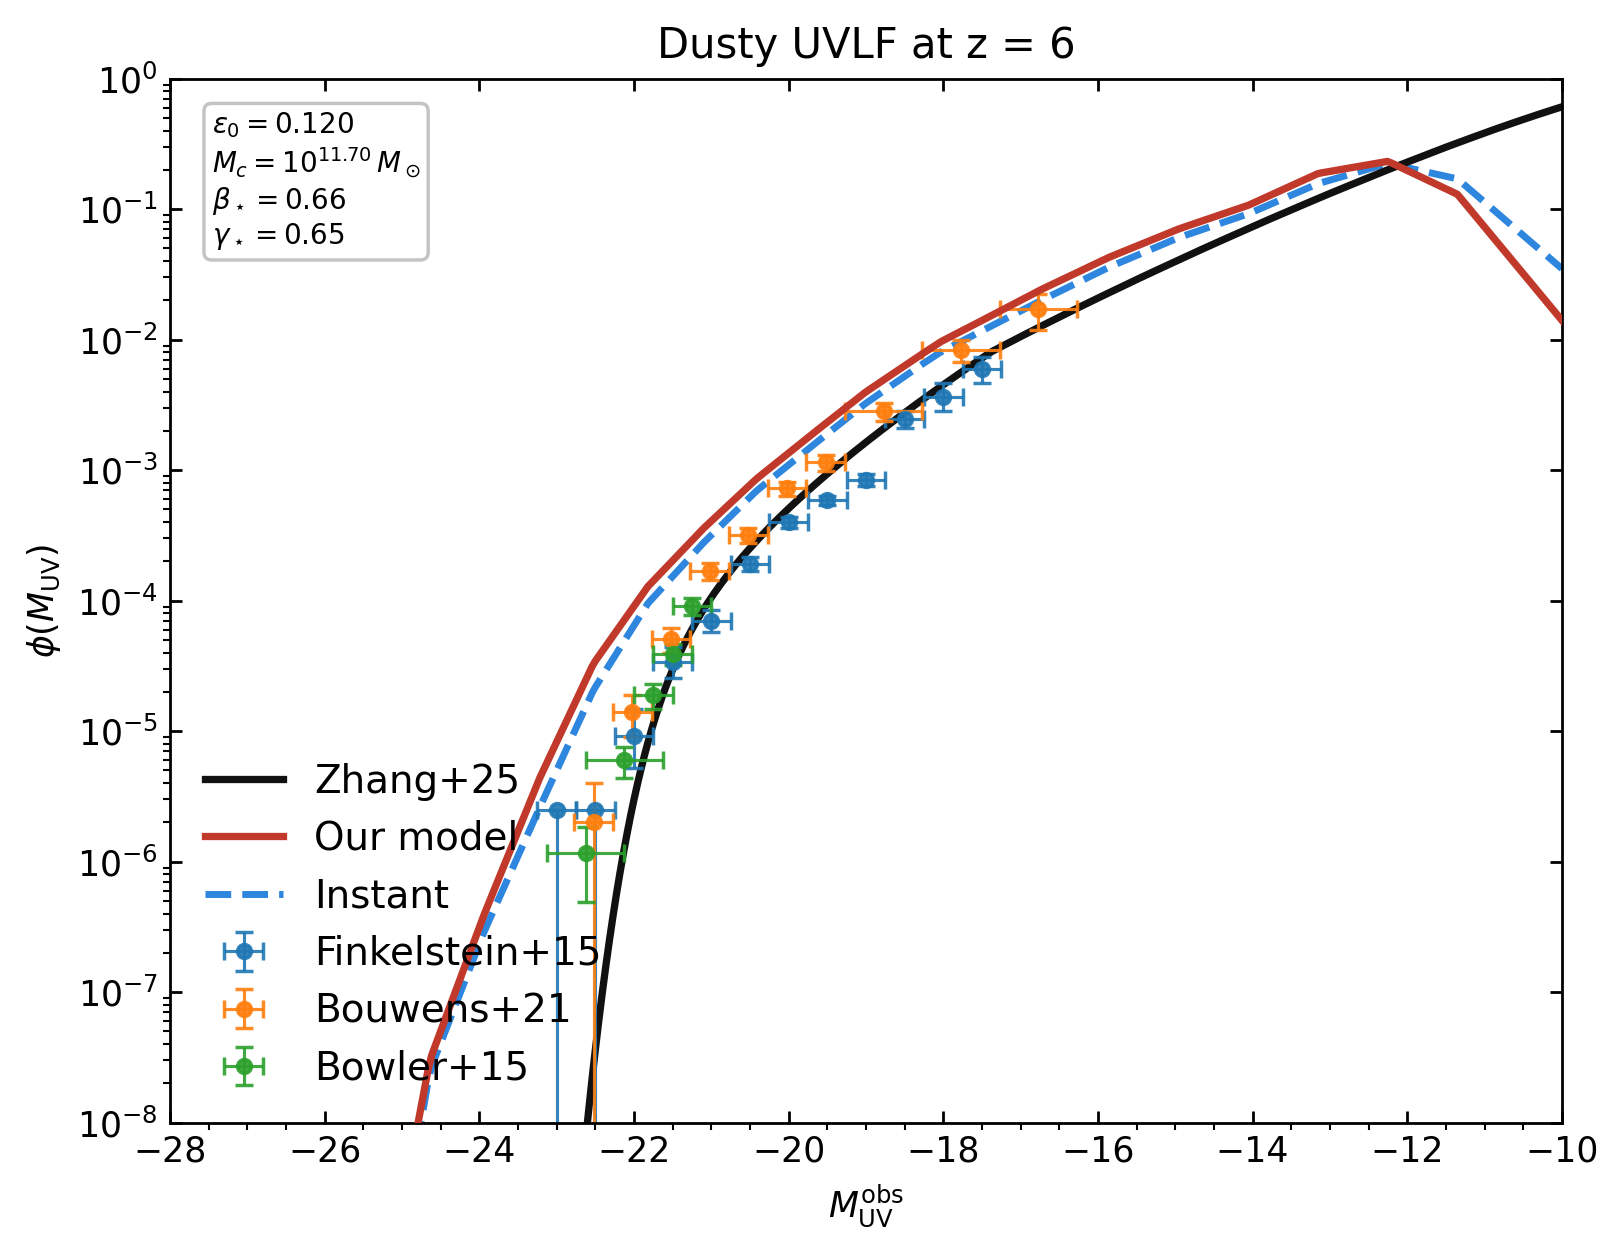
\includegraphics[width=0.97\linewidth]{uvlf_compare_no_puv_z6_dustonly.png}
  \vspace{-0.5em}
  {\large \(z=6\)}

  \column{0.5\textwidth}
  \centering
  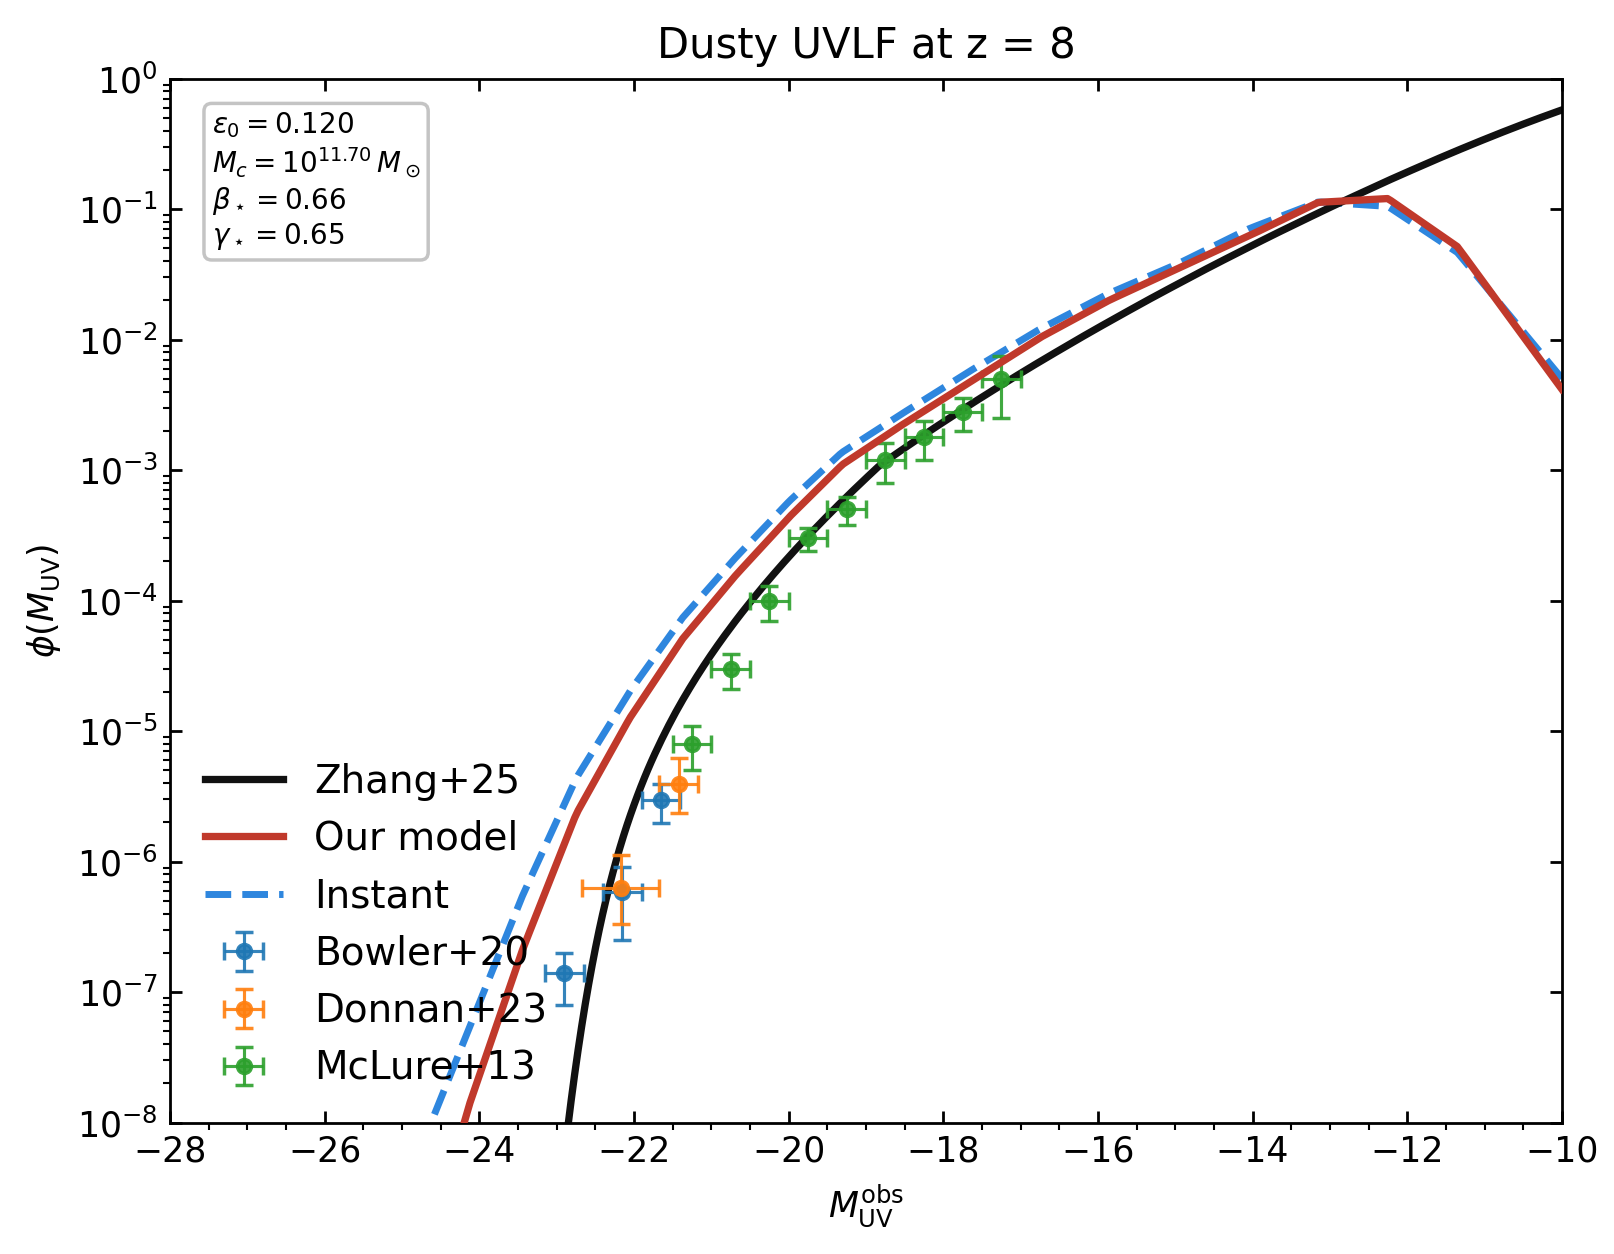
\includegraphics[width=0.97\linewidth]{uvlf_compare_no_puv_z8_dustonly.png}
  \vspace{-0.5em}
  {\large \(z=8\)}
\end{columns}
\end{frame}

\begin{frame}{同参数对比：\(z=10,12.5\)}
\begin{columns}[T,onlytextwidth]
  \column{0.5\textwidth}
  \centering
  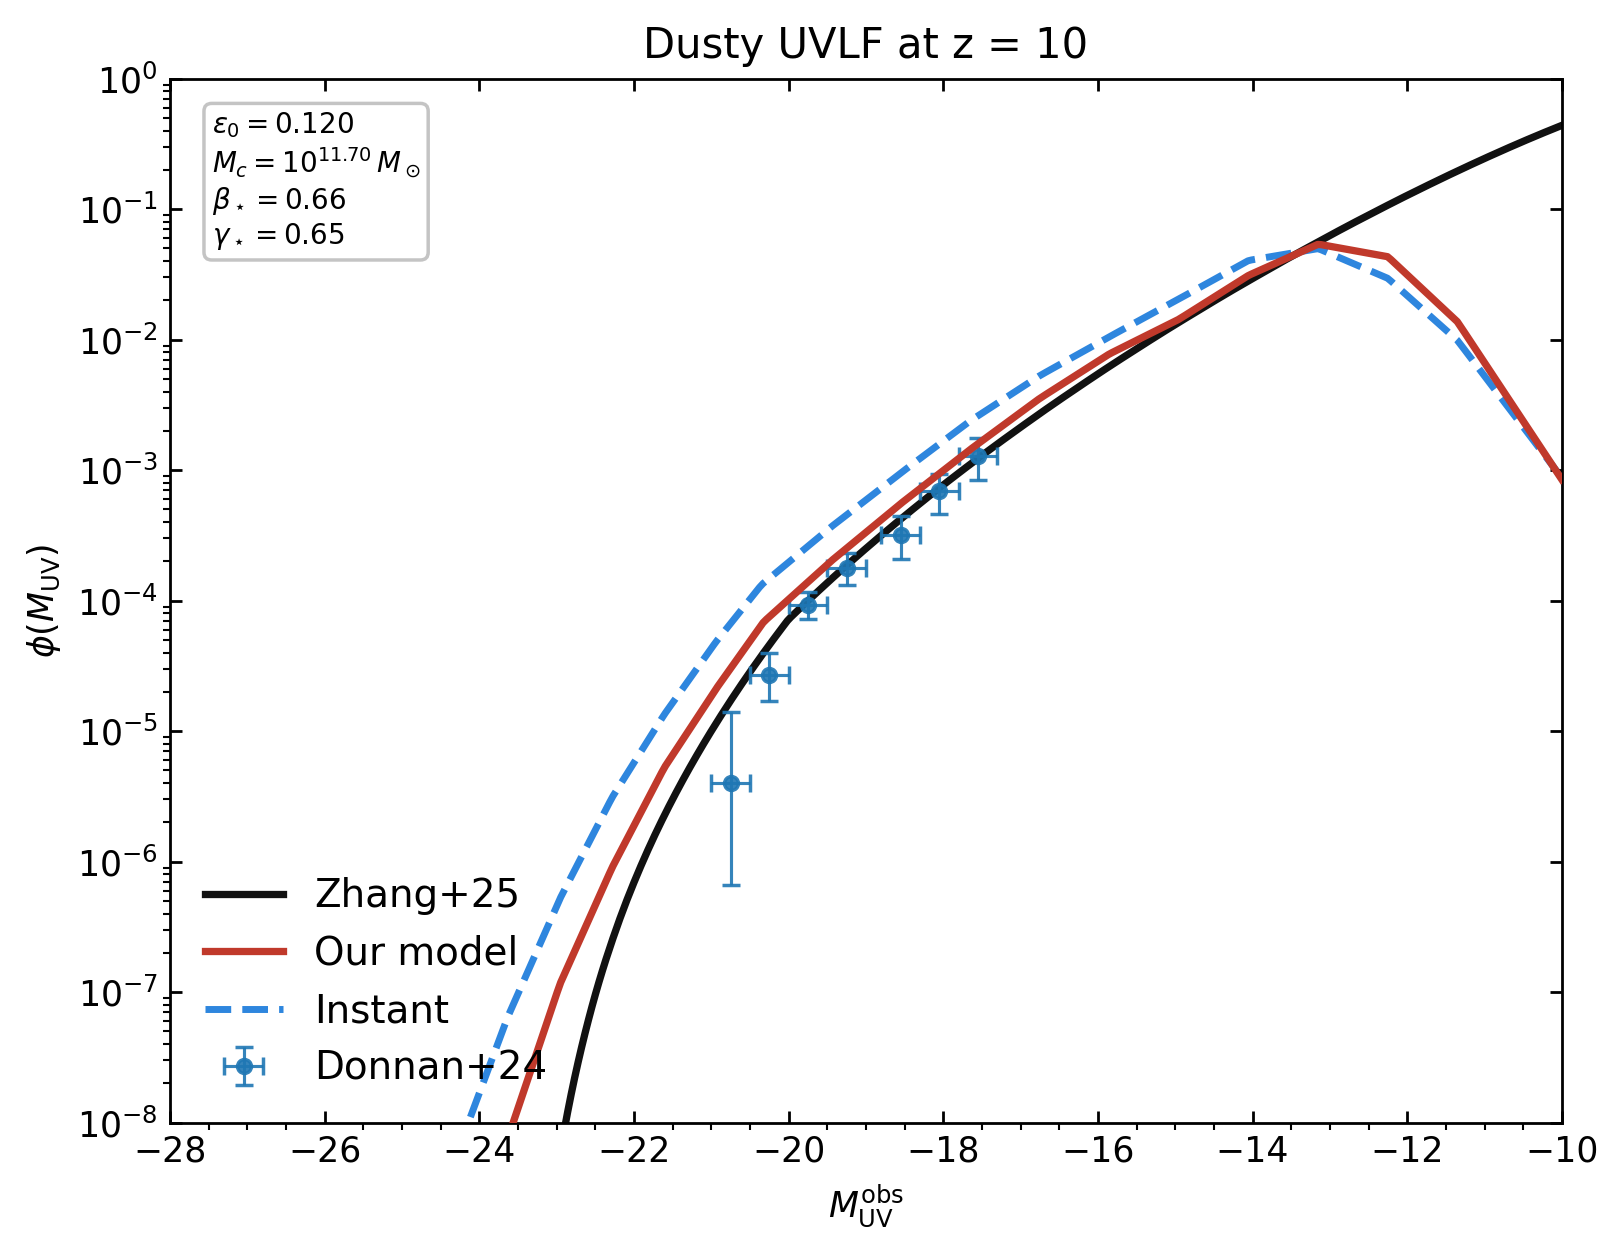
\includegraphics[width=0.97\linewidth]{uvlf_compare_no_puv_z10_dustonly.png}
  \vspace{-0.5em}
  {\large \(z=10\)}

  \column{0.5\textwidth}
  \centering
  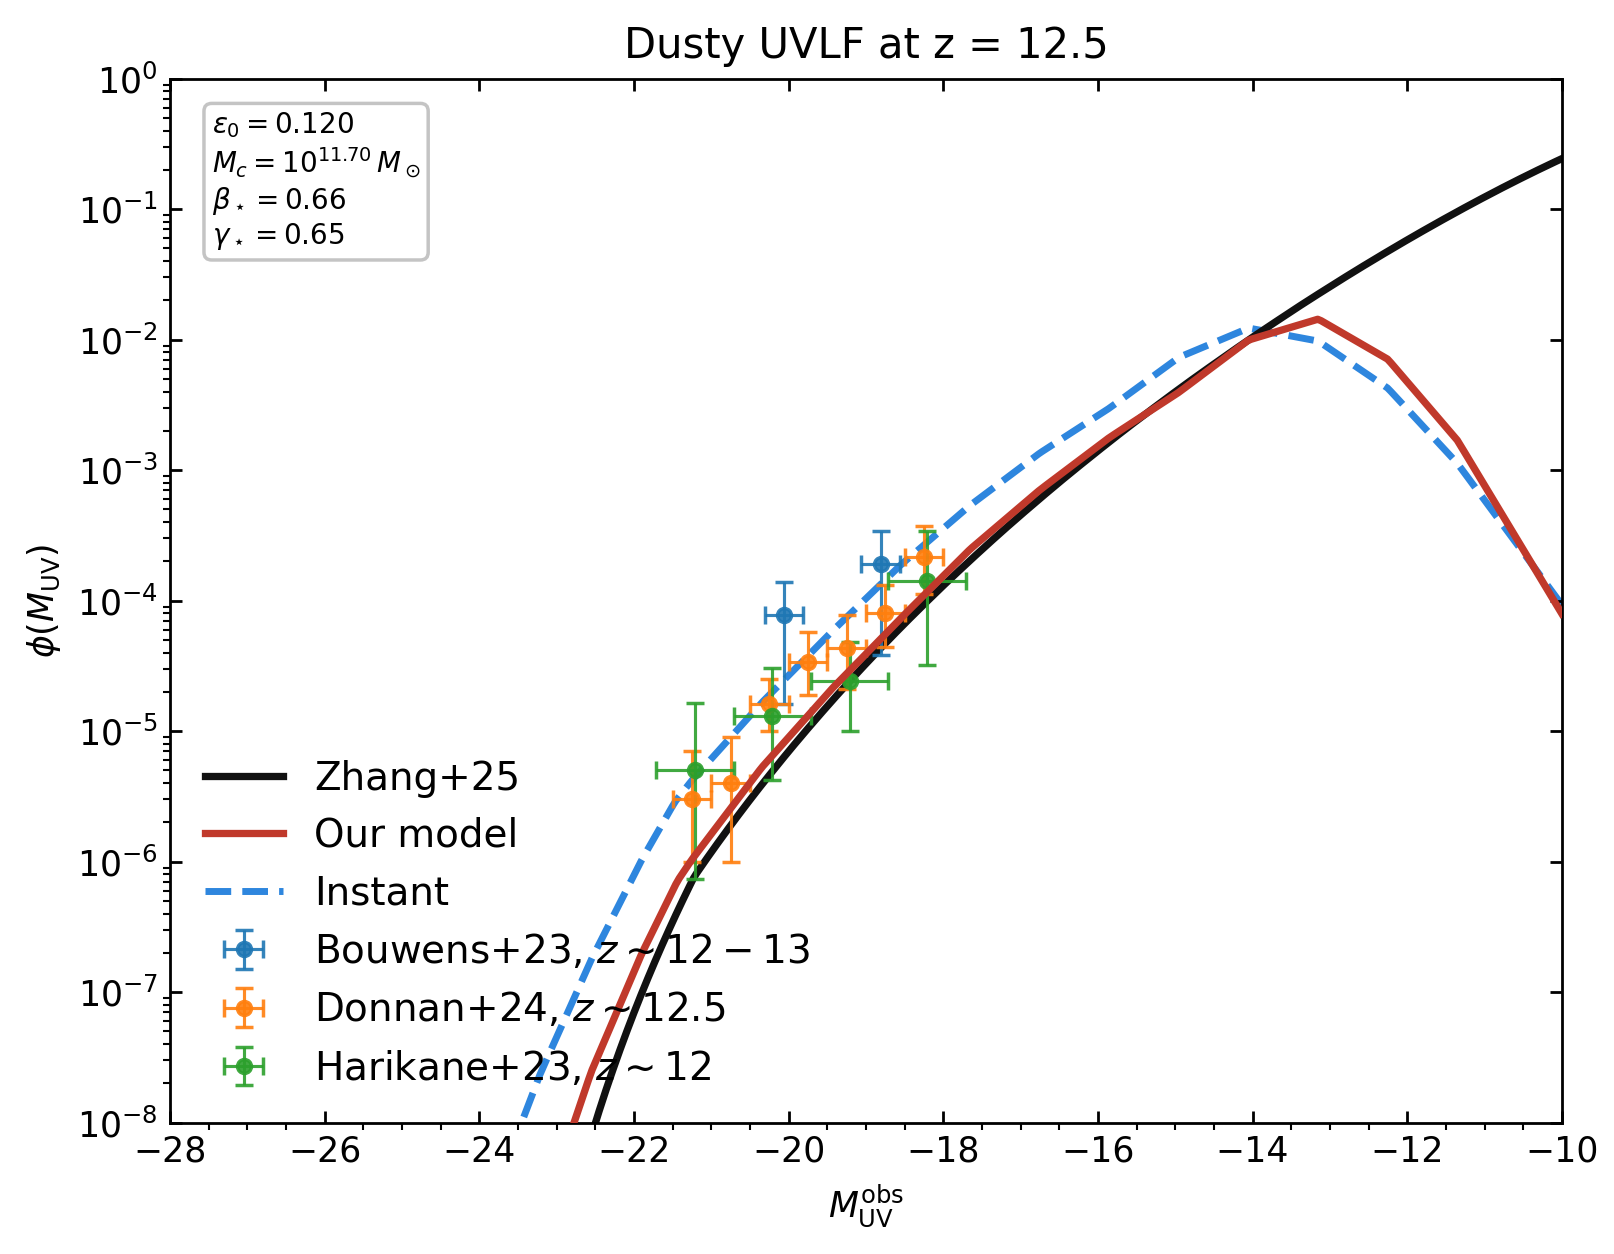
\includegraphics[width=0.97\linewidth]{uvlf_compare_no_puv_z12p5_dustonly.png}
  \vspace{-0.5em}
  {\large \(z=12.5\)}
\end{columns}
\end{frame}

\begin{frame}{为什么 \(L_{\rm UV}\) 的差距不等于 UVLF 的差距？}
\begin{columns}[T,onlytextwidth]
  \column{0.68\textwidth}
  \centering
  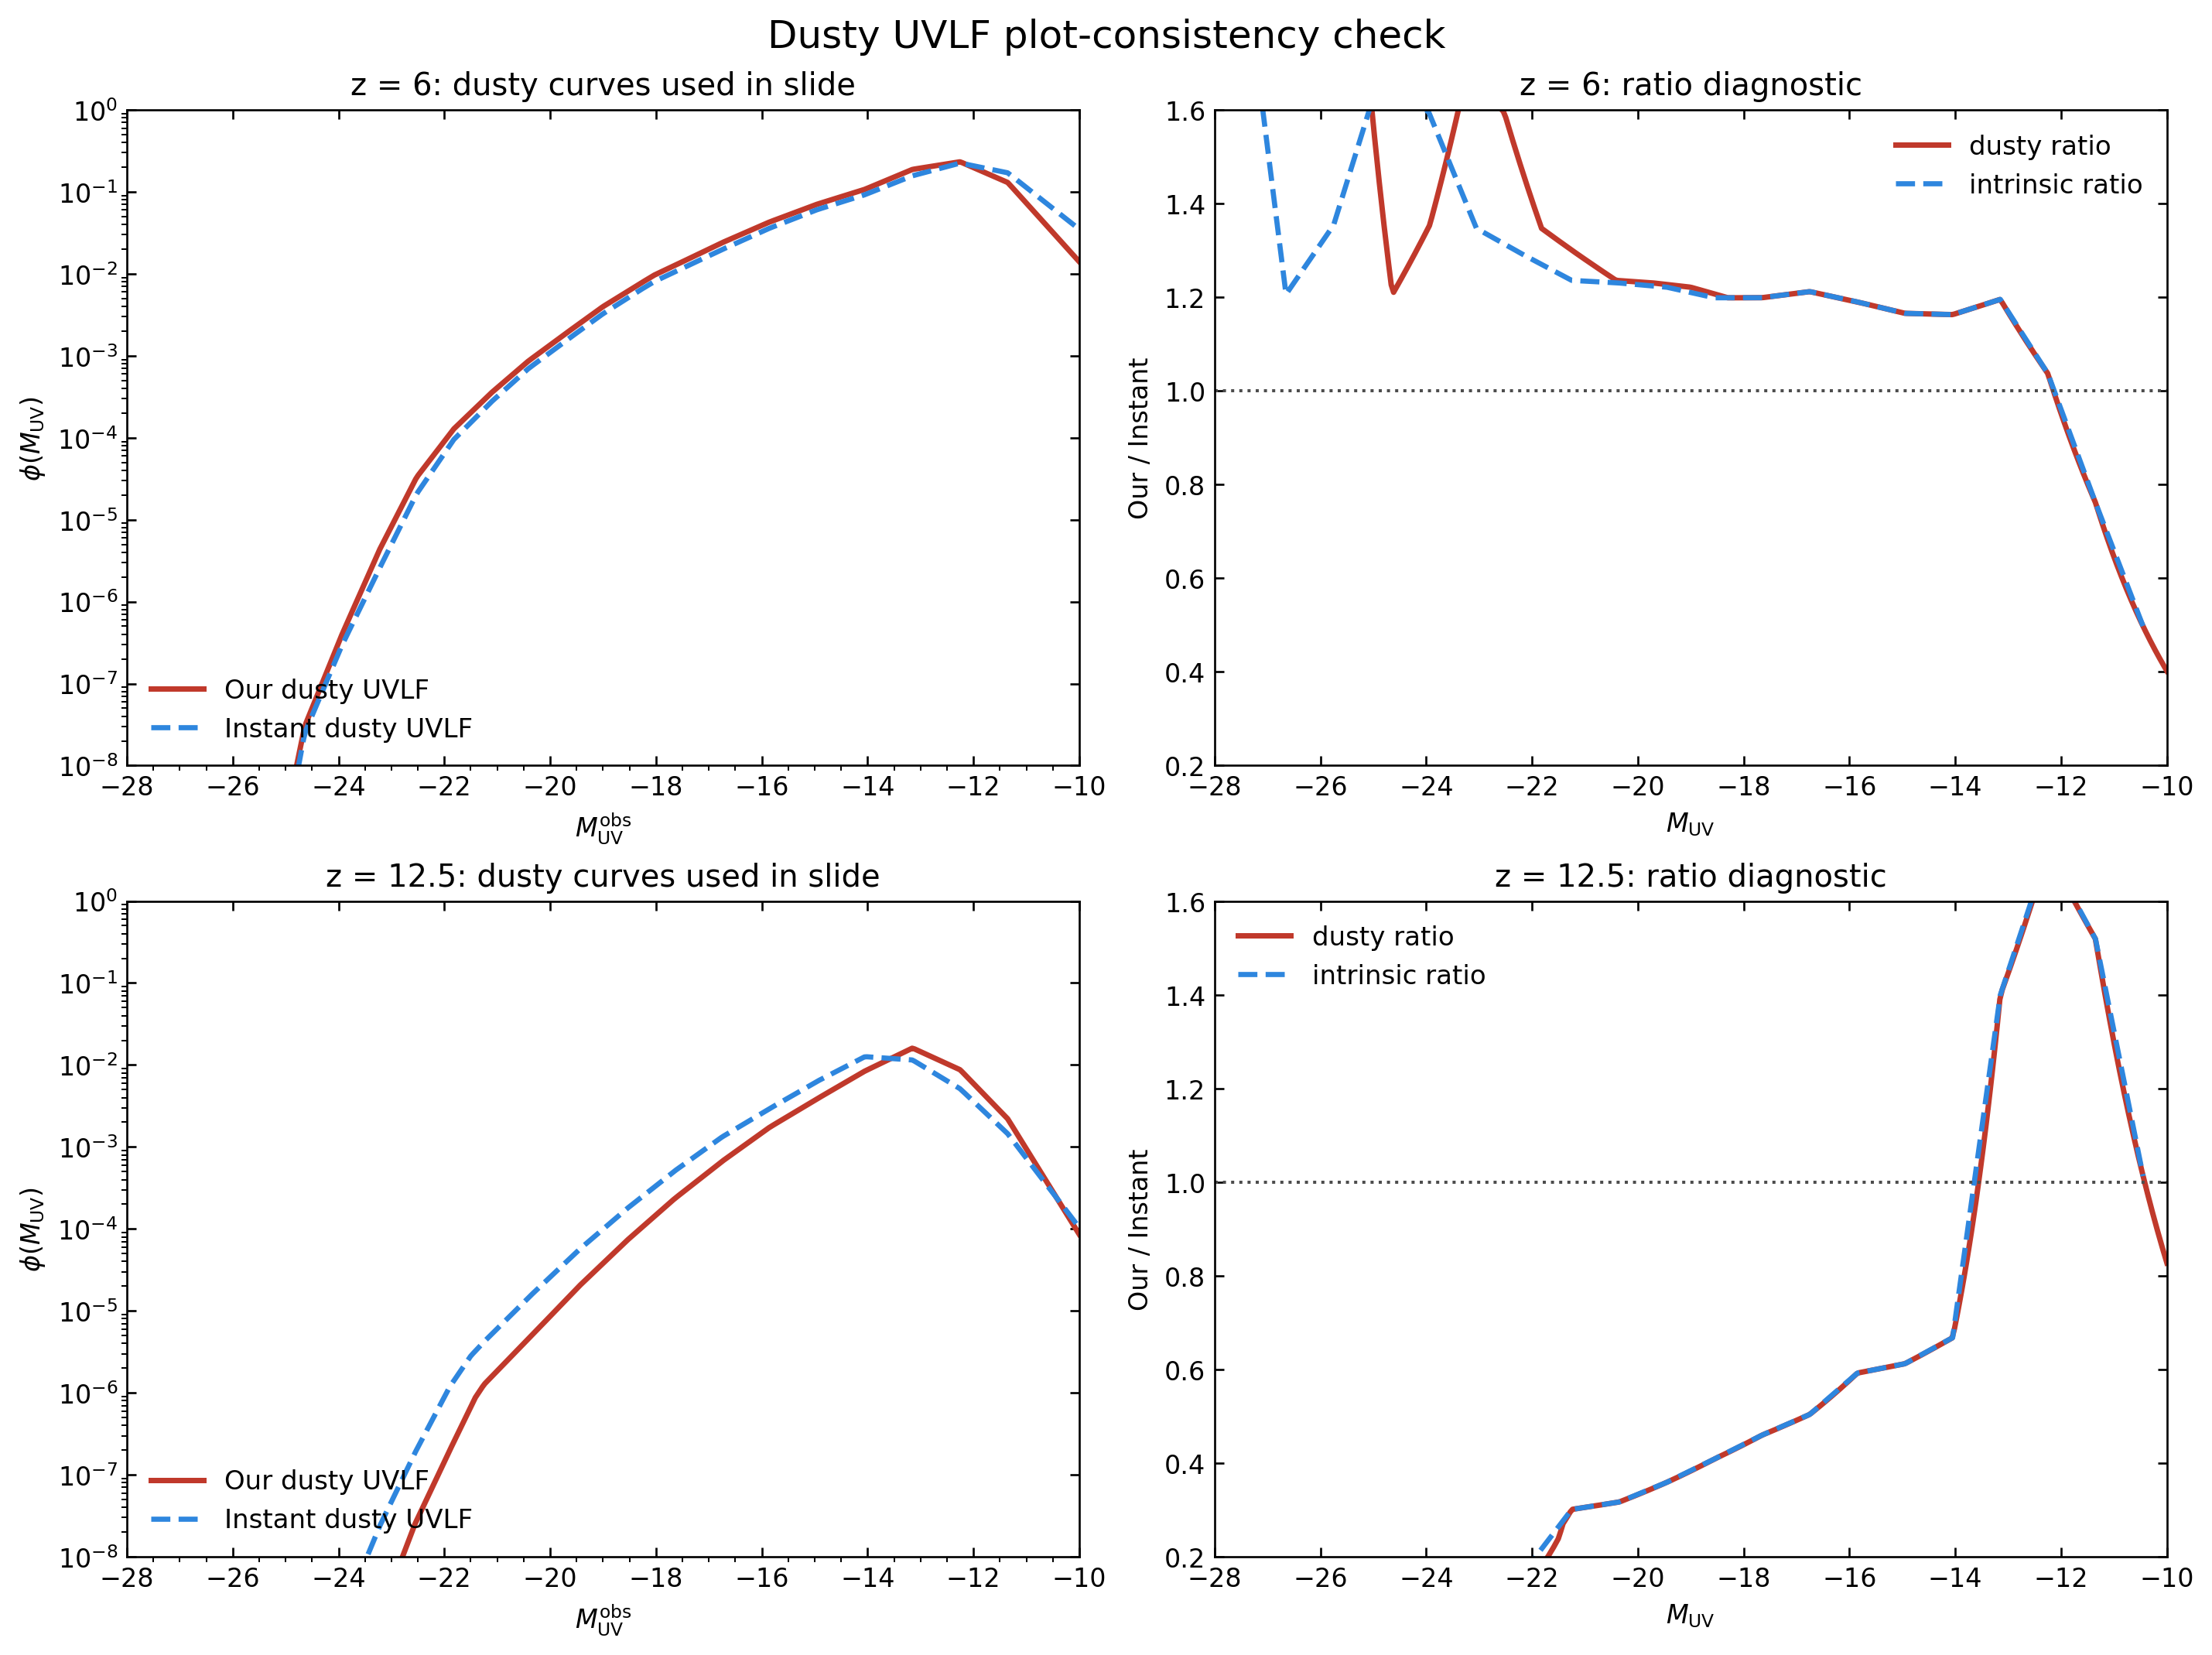
\includegraphics[width=\linewidth]{uvlf_plot_consistency_check_z6_12p5.png}

  \column{0.30\textwidth}
  \small
  \begin{beamercolorbox}[rounded=true, sep=0.55em, wd=\linewidth]{block body}
    \textbf{诊断结论}
    \begin{itemize}
      \item 单个 halo 的 \(L_{\rm UV}\) 比值，不会直接等于整条 UVLF 的 \(\phi\) 比值。
      \item UVLF 还要经过 HMF 权重与 \(P(M_{\rm UV}\mid M_{\rm h},z)\) 的映射。
      \item \(z=6\) 的 UVLF 中位比值约为 \(1.22\)，而 \(z=12.5\) 约为 \(0.38\)。
      \item dusty 与 intrinsic 比值几乎一致，因此 dust 不是主因。
    \end{itemize}
  \end{beamercolorbox}
\end{columns}
\end{frame}

\begin{frame}{SSP 相对瞬时 UV 基准的偏离}
\centering
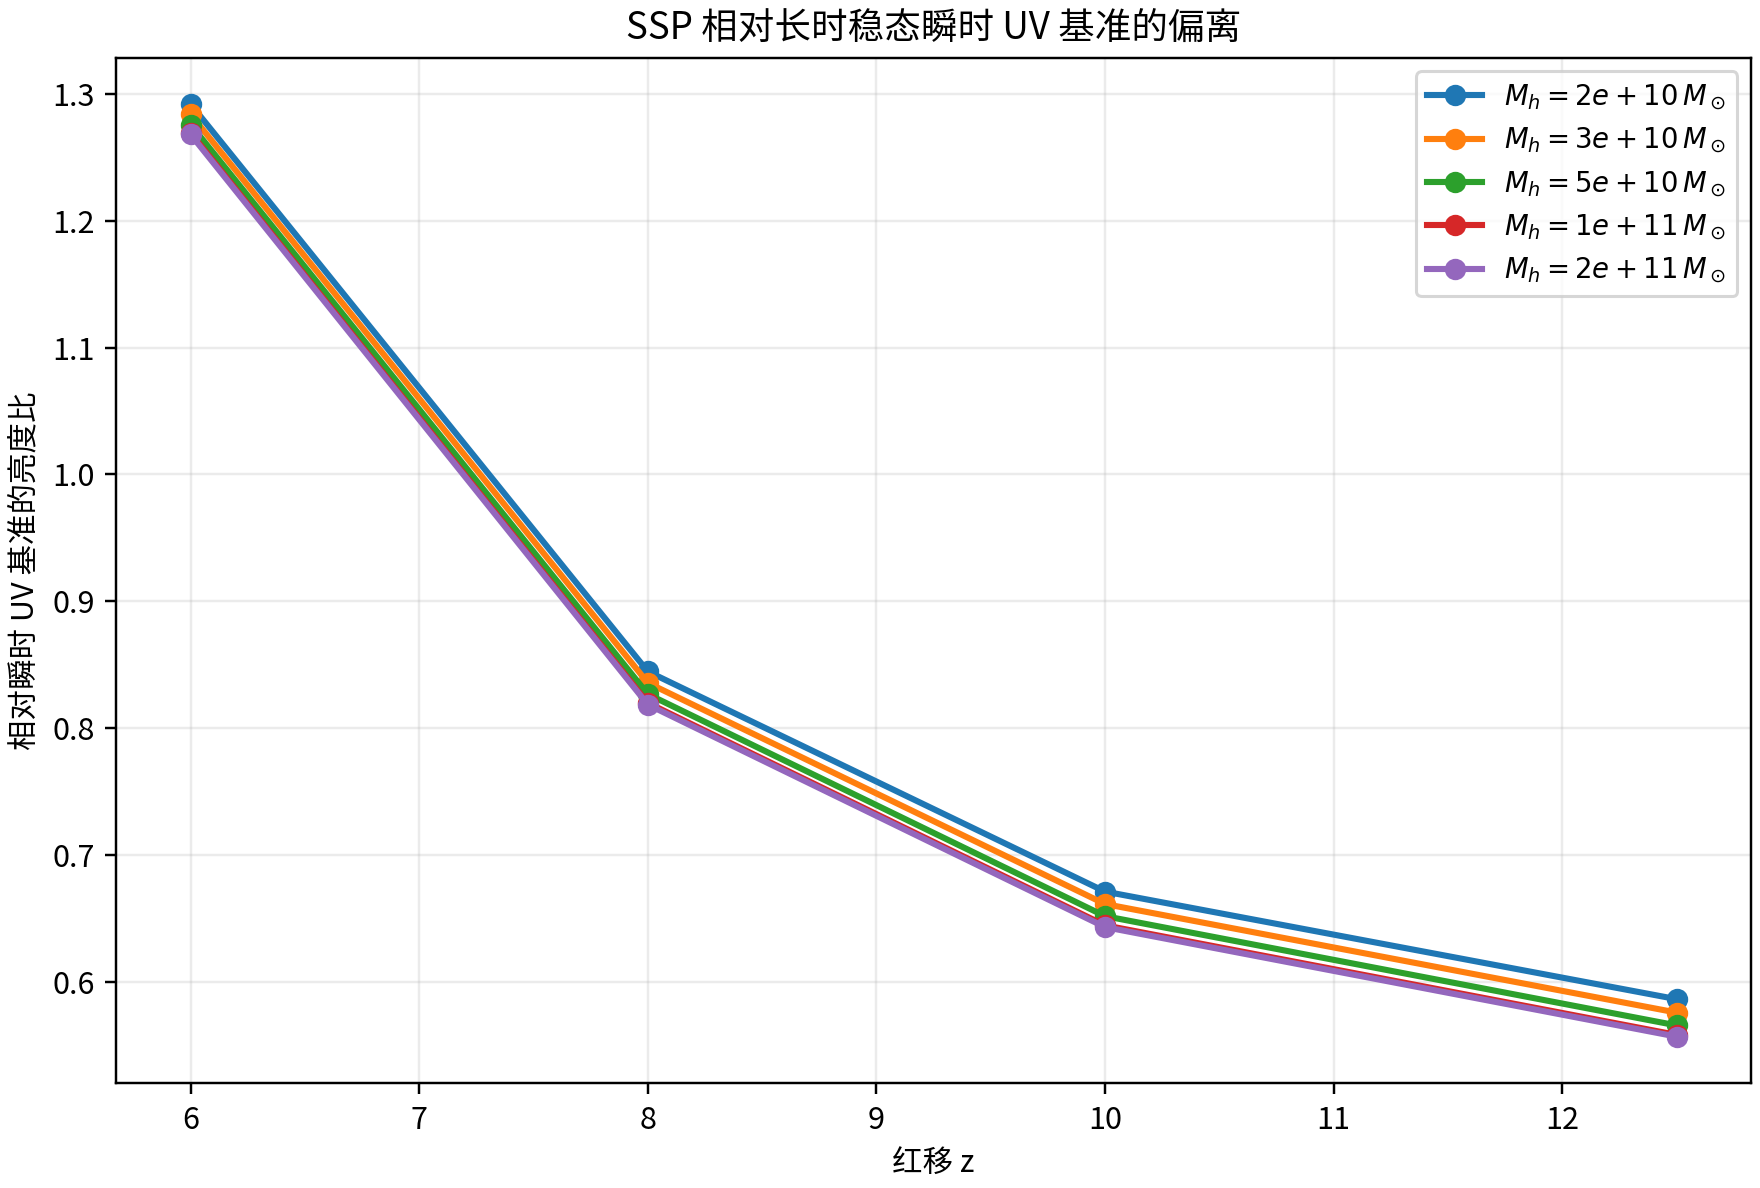
\includegraphics[width=0.64\linewidth]{ssp_vs_instant_ssplong_same_sfh.png}

\vspace{0.15em}
{\tiny 瞬时 UV 基准取 \(\mathrm{SFR}(z_{\rm obs}) / K_{\mathrm{UV,SSP,long}}\)（\(K_{\mathrm{UV,SSP,long}} \approx 6.1\times 10^{-29}\)）；比值小于 1 表示系统仍明显偏离长时稳态。}
\end{frame}

\begin{frame}{MAH / SFR 历史诊断}
\begin{columns}[T,onlytextwidth]
  \column{0.56\textwidth}
  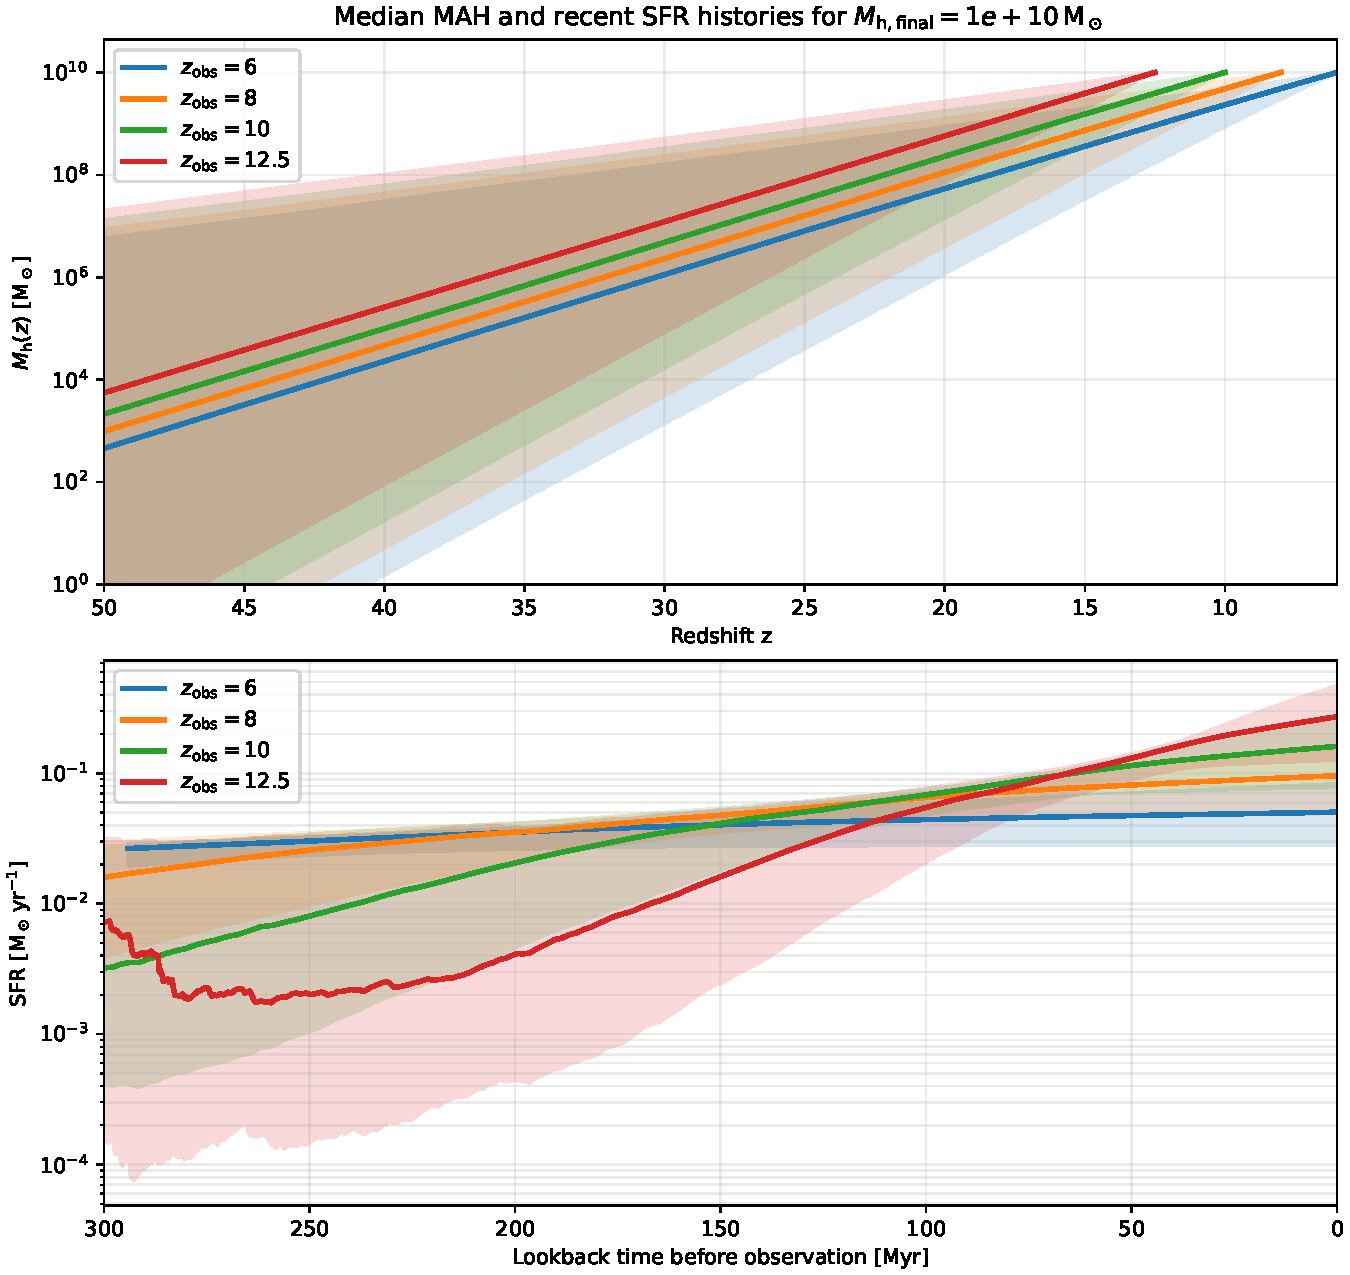
\includegraphics[width=\linewidth]{mah_sfr_four_z.pdf}

  \column{0.42\textwidth}
  \scriptsize
  \begin{align*}
  \langle \dot M \rangle_{\rm median}
  &= 24.1
  \left(\frac{M}{10^{12}M_\odot}\right)^{1.094} \\
  &\quad \times
  (1+1.75z)\sqrt{\Omega_m(1+z)^3+\Omega_\Lambda}
  \end{align*}

  \vspace{0.4em}
  \begin{beamercolorbox}[wd=\linewidth,sep=0.8em,rounded=true]{block body}
  \scriptsize
  对 \(M_{\rm h,final}=10^{10}M_\odot\)，当前 Monte Carlo 轨道给出的
  \(\dot M_{\rm h}\) 中位数与上式仅差约 \(3\%\)–\(4\%\)。

  \vspace{0.2em}
  \[
  \frac{\dot M_{\rm med}}{\dot M_{\rm formula}}
  =
  (0.959,\ 0.962,\ 0.969,\ 0.973)
  \]
  {\tiny 对应 \(z=6,8,10,12.5\)。}
  \end{beamercolorbox}
\end{columns}
\end{frame}

\begin{frame}{当前模型的主要问题}
\Large
\begin{itemize}
  \item 这张 SSP 表在长期恒定 SFR 极限下给出
  \[
    K_{\mathrm{UV,SSP,long}} \approx 6.1\times 10^{-29}
  \]
  明显小于 standard 的
  \[
    K_{\mathrm{UV,std}} = 1.17\times 10^{-28}
  \]
  \item 因而低红移 UV 会被系统性抬亮
  \item 用同一套 \(f_\star\) 同时拟合低 \(z\) 和高 \(z\) 时，当前 UV calibration 会放大 high-\(z\) tension
\end{itemize}
\end{frame}

\begin{frame}{结论}
\Large
\begin{itemize}
  \item 当前 pipeline 在形式上更物理，因为它使用了完整的 SSP 卷积
  \item 但当前 SSP UV calibration 在低红移给出更亮的 UV 归一化
  \item 这会放大跨红移联合拟合的 tension
\end{itemize}
\end{frame}

\end{document}
